\documentclass[notitlepage,groupedaddress]{IEEEtran}
%\documentclass{revtex4-1}
\usepackage{graphicx}
\usepackage{morefloats}
\usepackage{amsmath, amsthm, amssymb}
\usepackage{hyperref}
\usepackage{array}
\usepackage{subfig}
\usepackage{listings}
\usepackage{multirow}
\usepackage{booktabs}
%\pdfminorversion=4
\usepackage[font=small]{caption}
\hypersetup{colorlinks, linkcolor=blue,citecolor=blue, urlcolor=blue}
\newcommand{\ACK}{\emph{ACK}}
%\usepackage{cite}

% Default fixed font does not support bold face
\DeclareFixedFont{\ttb}{T1}{txtt}{bx}{n}{12} % for bold
\DeclareFixedFont{\ttm}{T1}{txtt}{m}{n}{12}  % for normal
\usepackage{color}
\definecolor{deepblue}{rgb}{0,0,0.5}
\definecolor{deepred}{rgb}{0.6,0,0}
\definecolor{deepgreen}{rgb}{0,0.5,0}
\newcommand{\fix}[1]{\texttt{\small #1}}
\newcommand{\sfix}[1]{\texttt{\scriptsize #1}}
\newcommand{\code}[1]{\texttt{\small #1}}

 

%\newcommand{\code}[2]{
%  \hrulefill
%  \subsection*{#1}
%  \lstinputlisting{#2}
%  \vspace{2em}
%}

\begin{document}
\title{ECE542 Mini-Project 1:\\ Analysis of Blue Waters Hardware Errors for
Weeks 40 and 41}
\author{Group 8: Matthew Tischer (tischer1), Zachary Estrada (zestrad2)}
%FIXME: Write your names, group name, data range in your dataset and the
%data-set assigned to you on the report.

\maketitle
%\begin{abstract}
%\end{abstract}


%\nocite{*}

\section{Task 0}

\subsection{Summarizing the Data Set}
In order to effectively summarize our data set, we used a few different techniques:

\begin{itemize}
\item The \fix{levels} function in R enumerates all of the different levels used in a factor.  In the case of the CompleteNode column, this allowed us to form a vector that represented every complete node name; by taking the length of this vector, we were able to determine the number of nodes in the system.  We also used this method to determine the unique number of machine check exception types.
\item As the data was ordered chronologically, the \fix{head} and \fix{tail} functions helped us to realize that eight days were represented in our data set.
\item The \fix{nrow} function returns the number of rows in a table.  We used this function to determine the total number of machine check exceptions and, after subsetting the data to only include rows where the \fix{ue} or \fix{ucc} bits were 1, the total number of uncorrectable errors in the data.
\end{itemize}

Our results are summarized in the following table:

\begin{table}[ht]
\centering
\begin{tabular}{rrrrrr}
  \hline
 & num\_nodes & num\_days & num\_entries & num\_uncorrectable\_errors & num\_machine\_check\_exception\_types \\ 
  \hline
1 & 910 & 8.00 & 16524 &   2 &  14 \\ 
   \hline
\end{tabular}
\end{table}

\subsection{Computing the MTBF}

Before we compute MTBFs in general, one note: we define MTBF throughout this report as the quantity $\frac{\textrm{length of measurement period}}{\textrm{number of failures}}$.  We define the measurement period as 8 full days, as we can count entries from eight different days in the data.  Note that we could have defined the measurement period as the time difference between the first and last failures; however, this method underestimates the MTBF more than our method because it ignores the failure-free time between the beginning (and end) of measurement and this data.

To calculate the MTBF of a particular type of node, I created the function \fix{get\_mtbf}, which returns the MTBF for our data set for nodes of a given type.  I accomplish this goal by subsetting the data (so that its \fix{nodeType} is what we desire), calculating the number of failures of the given type by using the \fix{nrow} function on the subsetted data, computing 8 days in seconds, and dividing the two quantities to determine a MTBF value.  The function can also accept a boolean \fix{all} argument, which controls whether all of the data should be used in the analysis.  If \fix{all} is \fix{TRUE}, the data is not subsetted; this functionality was added to easily support determining the MTBF for all nodes at once.

I then create a data frame with all of my results by iterating over all node types and adding their MTBFs and type data.  I also create an entry for all types and call the \fix{get\_mtbf} function with the \fix{all} argument set to \fix{TRUE} to calculate the MTBF for all node types.

The results of this section are summarized in the following table:

\begin{table}[ht]
\centering
\begin{tabular}{rlr}
  \hline
 & nodeType & mtbf \\ 
  \hline
1 & compute & 0.02 \\ 
  2 & GPU & 0.28 \\ 
  3 & lnet & 17.45 \\ 
  4 & service & 0.05 \\ 
  5 & mom & 2.46 \\ 
  6 & all & 0.01 \\ 
   \hline
\end{tabular}
\end{table}

\section{Task 1}

\subsection{Distribution of Machine Check Exceptions}

In order to compare this distribution of machine check exceptions across all node types, we first must define what we consider ``memory'', ``L1'' and ``L2'' errors.  For the purposes of this (and future) problems, we define:

\begin{verbatim}
L1_errors <- c("L1 cache Fill ECC error", "L1 tag load", "L1 TLB IC load")
L2_errors <- c("L2 cache Fill ECC error", "L2 cache Fill ECC Error", "L2 ECC Error", "L2 IC cache parity error", "L2 TLB")
mem_errors <- c("DRAM Parity Error", "ECC Error")
\end{verbatim}

We do not include \fix{"NB Array Error"} in any of these categories, as the AMD manual explicitly distinguishes between the northbridge and memory.  The \fix{"Table Walk Data Error"}, \fix{"Data copy back Evict"}, and \fix{"Link Retry"} errors do not directly involve the main memory, L1, or L2 caches.

Once we defined these categories, we filtered the data by both type and node type and used \fix{nrow} to determine the number (and, by dividing, percentage) of entries in each category.

The results of this distribution exercise are shown below:

\begin{table}[ht]
\centering
\begin{tabular}{rllrr}
  \hline
 & nodeType & type & nerr & perr \\ 
  \hline
1 & compute & L1 & 210 & 0.02 \\ 
  2 & compute & L2 & 177 & 0.01 \\ 
  3 & compute & mem & 8848 & 0.74 \\ 
  4 & compute & other & 2685 & 0.23 \\ 
  5 & GPU & L1 &   2 & 0.00 \\ 
  6 & GPU & L2 &  14 & 0.02 \\ 
  7 & GPU & mem & 616 & 0.91 \\ 
  8 & GPU & other &  48 & 0.07 \\ 
  9 & lnet & L1 &   0 & 0.00 \\ 
  10 & lnet & L2 &   0 & 0.00 \\ 
  11 & lnet & mem &   7 & 0.64 \\ 
  12 & lnet & other &   4 & 0.36 \\ 
  13 & service & L1 &   4 & 0.00 \\ 
  14 & service & L2 &  38 & 0.01 \\ 
  15 & service & mem & 2382 & 0.62 \\ 
  16 & service & other & 1411 & 0.37 \\ 
  17 & mom & L1 &   0 & 0.00 \\ 
  18 & mom & L2 &   0 & 0.00 \\ 
  19 & mom & mem &  76 & 0.97 \\ 
  20 & mom & other &   2 & 0.03 \\ 
  21 & all & L1 & 216 & 0.01 \\ 
  22 & all & L2 & 229 & 0.01 \\ 
  23 & all & mem & 11929 & 0.72 \\ 
  24 & all & other & 4150 & 0.25 \\ 
   \hline
\end{tabular}
\end{table}

Generally speaking, memory errors account for the majority of errors encountered in the data, while L1 and L2 cache errors are relatively rare.

To compute the MTBFs across banks and these extended types, we used the same formula discussed in Task 0 to calculate the MTBF across the subsetted data set.

The results of this experiment are shown below:

\begin{table}[ht]
\centering
\begin{tabular}{rrllr}
  \hline
 & bank & nodeType & type & mtbf \\ 
  \hline
1 &   4 & compute & L1 & Inf \\ 
  2 &   4 & compute & L2 & Inf \\ 
  3 &   4 & compute & mem & 0.02 \\ 
  4 &   4 & compute & other & 0.07 \\ 
  5 &   4 & GPU & L1 & Inf \\ 
  6 &   4 & GPU & L2 & Inf \\ 
  7 &   4 & GPU & mem & 0.31 \\ 
  8 &   4 & GPU & other & 4.00 \\ 
  9 &   4 & lnet & L1 & Inf \\ 
  10 &   4 & lnet & L2 & Inf \\ 
  11 &   4 & lnet & mem & 27.43 \\ 
  12 &   4 & lnet & other & 48.00 \\ 
  13 &   4 & service & L1 & Inf \\ 
  14 &   4 & service & L2 & Inf \\ 
  15 &   4 & service & mem & 0.08 \\ 
  16 &   4 & service & other & 0.14 \\ 
  17 &   4 & mom & L1 & Inf \\ 
  18 &   4 & mom & L2 & Inf \\ 
  19 &   4 & mom & mem & 2.53 \\ 
  20 &   4 & mom & other & 96.00 \\ 
  21 &   4 & all & L1 & Inf \\ 
  22 &   4 & all & L2 & Inf \\ 
  23 &   4 & all & mem & 0.02 \\ 
  24 &   4 & all & other & 0.05 \\ 
  25 &   1 & compute & L1 & 0.96 \\ 
  26 &   1 & compute & L2 & 14.77 \\ 
  27 &   1 & compute & mem & Inf \\ 
  28 &   1 & compute & other & Inf \\ 
  29 &   1 & GPU & L1 & 192.00 \\ 
  30 &   1 & GPU & L2 & Inf \\ 
  31 &   1 & GPU & mem & Inf \\ 
  32 &   1 & GPU & other & Inf \\ 
  33 &   1 & lnet & L1 & Inf \\ 
  34 &   1 & lnet & L2 & Inf \\ 
  35 &   1 & lnet & mem & Inf \\ 
  36 &   1 & lnet & other & Inf \\ 
  37 &   1 & service & L1 & 96.00 \\ 
  38 &   1 & service & L2 & Inf \\ 
  39 &   1 & service & mem & Inf \\ 
  40 &   1 & service & other & Inf \\ 
  41 &   1 & mom & L1 & Inf \\ 
  42 &   1 & mom & L2 & Inf \\ 
  43 &   1 & mom & mem & Inf \\ 
  44 &   1 & mom & other & Inf \\ 
  45 &   1 & all & L1 & 0.95 \\ 
  46 &   1 & all & L2 & 14.77 \\ 
  47 &   1 & all & mem & Inf \\ 
  48 &   1 & all & other & Inf \\ 
  49 &   2 & compute & L1 & 32.00 \\ 
  50 &   2 & compute & L2 & 1.17 \\ 
  51 &   2 & compute & mem & Inf \\ 
  52 &   2 & compute & other & 192.00 \\ 
  53 &   2 & GPU & L1 & Inf \\ 
  54 &   2 & GPU & L2 & 13.71 \\ 
  55 &   2 & GPU & mem & Inf \\ 
  56 &   2 & GPU & other & Inf \\ 
  57 &   2 & lnet & L1 & Inf \\ 
  58 &   2 & lnet & L2 & Inf \\ 
  59 &   2 & lnet & mem & Inf \\ 
  60 &   2 & lnet & other & Inf \\ 
  61 &   2 & service & L1 & 96.00 \\ 
  62 &   2 & service & L2 & 5.05 \\ 
  63 &   2 & service & mem & Inf \\ 
  64 &   2 & service & other & Inf \\ 
  65 &   2 & mom & L1 & Inf \\ 
  66 &   2 & mom & L2 & Inf \\ 
  67 &   2 & mom & mem & Inf \\ 
  68 &   2 & mom & other & Inf \\ 
  69 &   2 & all & L1 & 24.00 \\ 
  70 &   2 & all & L2 & 0.89 \\ 
  71 &   2 & all & mem & Inf \\ 
  72 &   2 & all & other & 192.00 \\ 
  73 &   0 & compute & L1 & 48.00 \\ 
  74 &   0 & compute & L2 & Inf \\ 
  75 &   0 & compute & mem & Inf \\ 
  76 &   0 & compute & other & Inf \\ 
  77 &   0 & GPU & L1 & 192.00 \\ 
  78 &   0 & GPU & L2 & Inf \\ 
  79 &   0 & GPU & mem & Inf \\ 
  80 &   0 & GPU & other & Inf \\ 
  81 &   0 & lnet & L1 & Inf \\ 
  82 &   0 & lnet & L2 & Inf \\ 
  83 &   0 & lnet & mem & Inf \\ 
  84 &   0 & lnet & other & Inf \\ 
  85 &   0 & service & L1 & Inf \\ 
  86 &   0 & service & L2 & Inf \\ 
  87 &   0 & service & mem & Inf \\ 
  88 &   0 & service & other & Inf \\ 
  89 &   0 & mom & L1 & Inf \\ 
  90 &   0 & mom & L2 & Inf \\ 
  91 &   0 & mom & mem & Inf \\ 
  92 &   0 & mom & other & Inf \\ 
  93 &   0 & all & L1 & 38.40 \\ 
  94 &   0 & all & L2 & Inf \\ 
  95 &   0 & all & mem & Inf \\ 
  96 &   0 & all & other & Inf \\ 
   \hline
\end{tabular}
\end{table}


Note that the MTBFs across different node types are very different: the MTBF for bank 4 memory errors varies from about 0.02 hours (\fix{compute}) to about 27 hours (\fix{lnet}).  There are a few possibilities for the cause of these results:

\begin{itemize}
\item Different types of nodes have different quantities of memory and cache; if more memory is present, MTBFs should be lower as there are more components that can fail.
\item Different types of nodes have different utilization percentages: it is possible that the routing nodes (\fix{lnet, mom}) are used less relative to their maximum capacity versus compute nodes (for example), leading to smaller MTBFs.
\end{itemize}

There are two uncorrectable errors in our data set, yielding an MTBF of 96 hours and a FIT of approximately $1.042 \cdot 10^7$.  One error occured in bank 0 of a compute node and was an L1 error, while the second error occured in bank 4 of a compute node and was a memory error.  If we wish to separate the uncorrectable errors by bank, node type, or type, the two resulting entries would individually have MTBF values of 192 hours and FIT values of $5.208 \cdot 10^6$.

\subsection{Time Between Consecutive Failures}
\subsubsection{Plotting the Daily MTBF}

In order to compute the MTBF per day, we can subset the data by days.  The easiest way to do this is to convert ``October 6, 2012 12:00 AM CDT'' into a Unix timestamp and use the fact that there are 86,400 seconds in a day to create upper and lower bounds for a given day's timestamp.  Once we have filtered this data, we can calculate MTBF by dividing 86400 seconds by the number of failures in the filtered data.  By concatenating the results for every day together, we can plot this data on a graph.

The graphs for each day are shown below:

\begin{figure}[h]
\centering
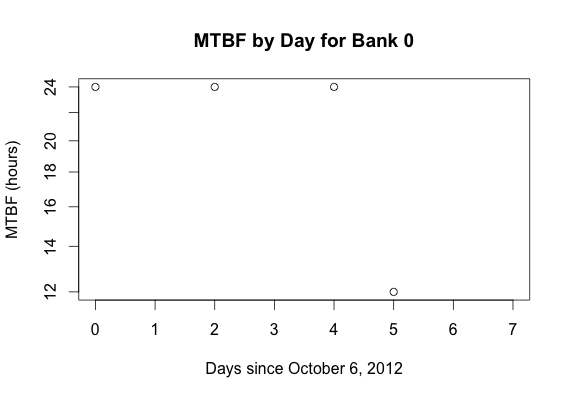
\includegraphics{images/mtbf_0.png}
\end{figure}

\begin{figure}[h]
\centering
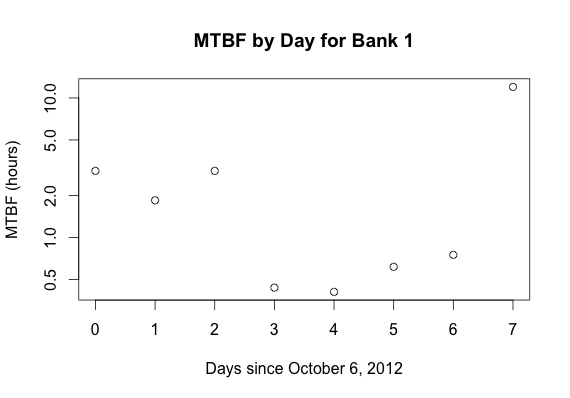
\includegraphics{images/mtbf_1.png}
\end{figure}

\begin{figure}[h]
\centering
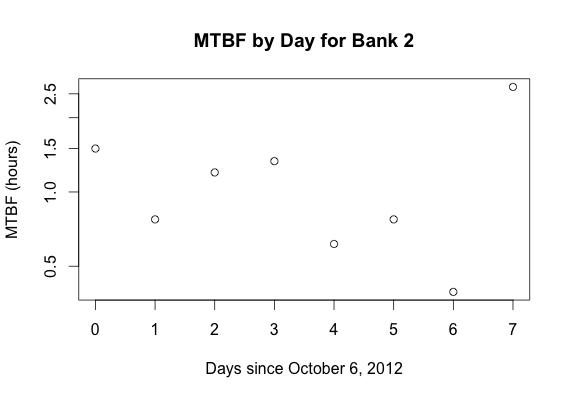
\includegraphics{images/mtbf_2.png}
\end{figure}

\begin{figure}[h]
\centering
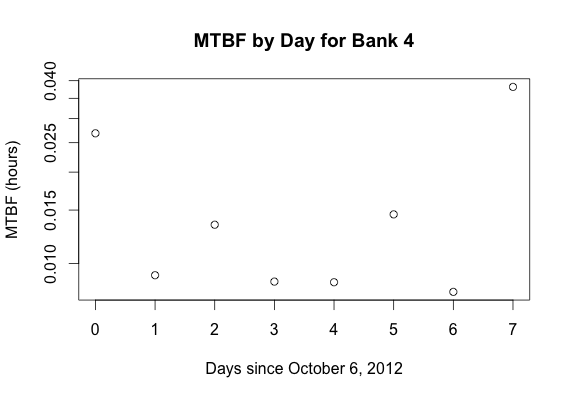
\includegraphics{images/mtbf_4.png}
\end{figure}

\subsubsection{Plotting the TBFs}

The \fix{diff} command can be used on a vector of numeric values to return the differences between subsequent values.  If we call \fix{diff} on a set of filtered data, we can use the \fix{hist} command to visualize the time between failures.

The plots for the TBFs are shown below.  Note that we do not create a histogram for categories that only have one point of data in them (as it is impossible to create a sensible time between failure amount there)--as a result, the graph for all node types may differ significantly from the individual graph categories due to the addition of these one-item categories.


\begin{figure}[h]
\centering
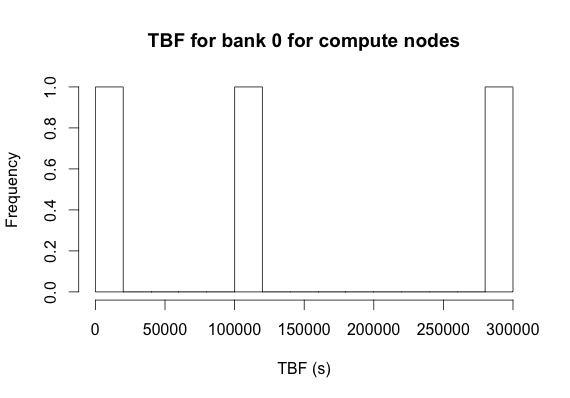
\includegraphics{images/tbf_0_c.png}
\end{figure}

\begin{figure}[h]
\centering
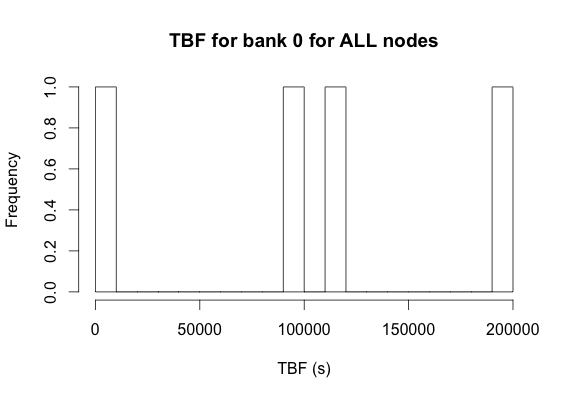
\includegraphics{images/tbf_0_a.png}
\end{figure}

\begin{figure}[h]
\centering
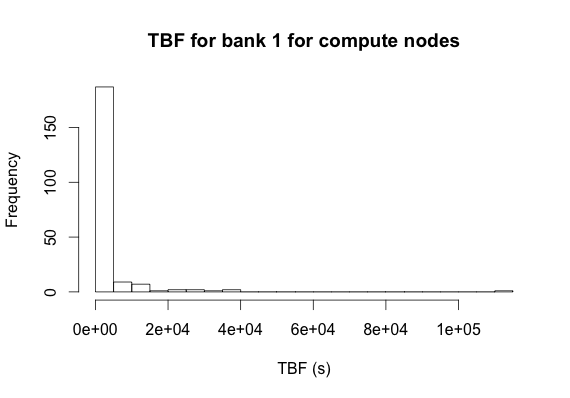
\includegraphics{images/tbf_1_c.png}
\end{figure}

\begin{figure}[h]
\centering
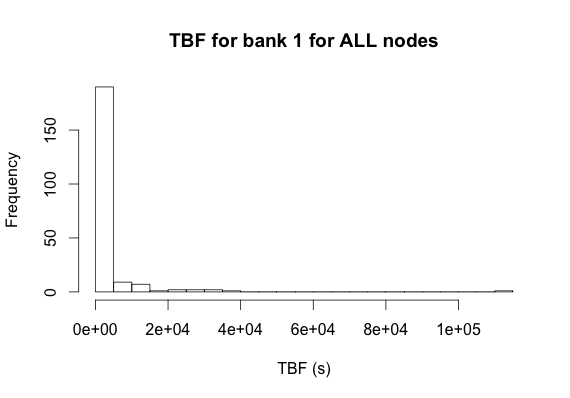
\includegraphics{images/tbf_1_a.png}
\end{figure}

\begin{figure}[h]
\centering
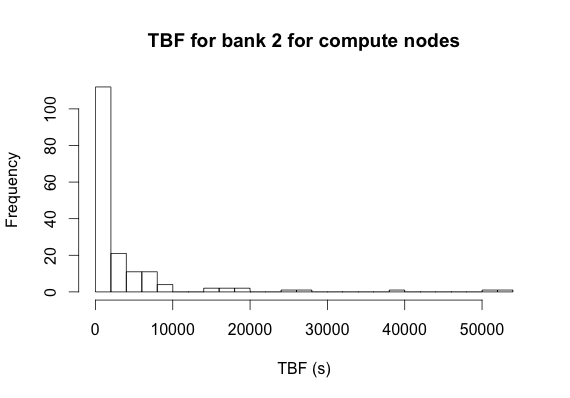
\includegraphics{images/tbf_2_c.png}
\end{figure}

\begin{figure}[h]
\centering
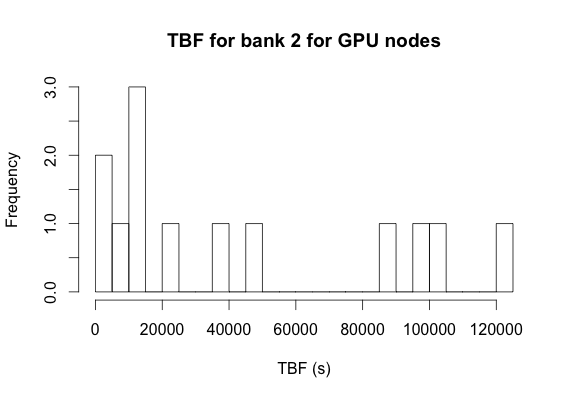
\includegraphics{images/tbf_2_g.png}
\end{figure}

\begin{figure}[h]
\centering
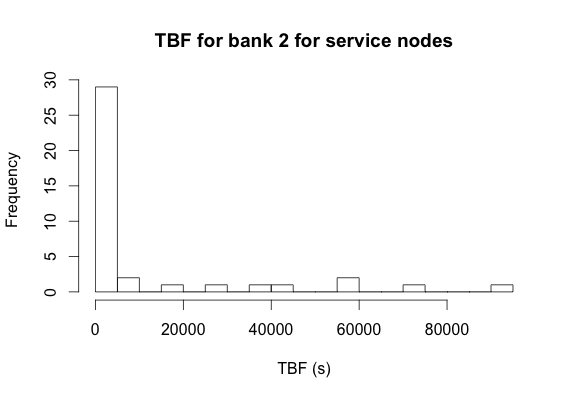
\includegraphics{images/tbf_2_s.png}
\end{figure}

\begin{figure}[h]
\centering
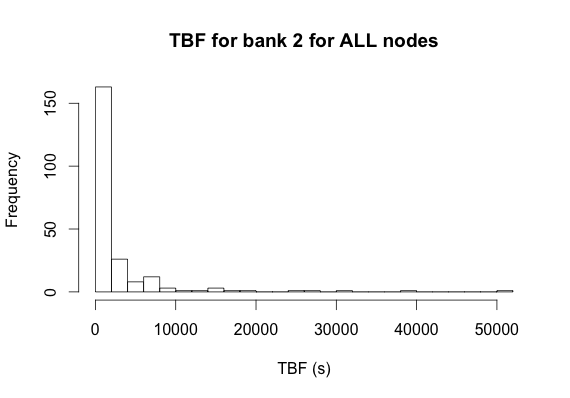
\includegraphics{images/tbf_2_a.png}
\end{figure}

\begin{figure}[h]
\centering
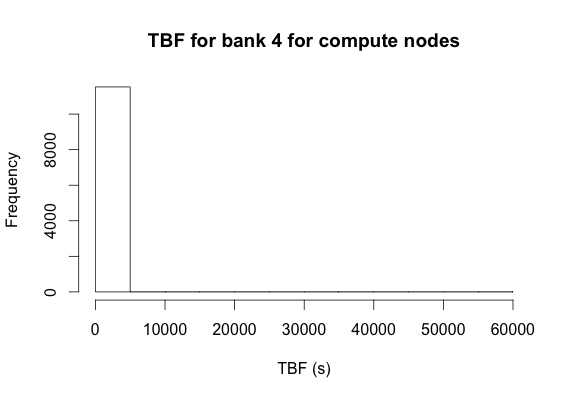
\includegraphics{images/tbf_4_c.png}
\end{figure}

\begin{figure}[h]
\centering
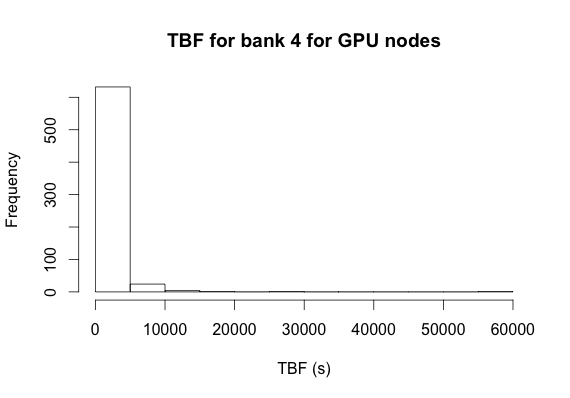
\includegraphics{images/tbf_4_g.png}
\end{figure}

\begin{figure}[h]
\centering
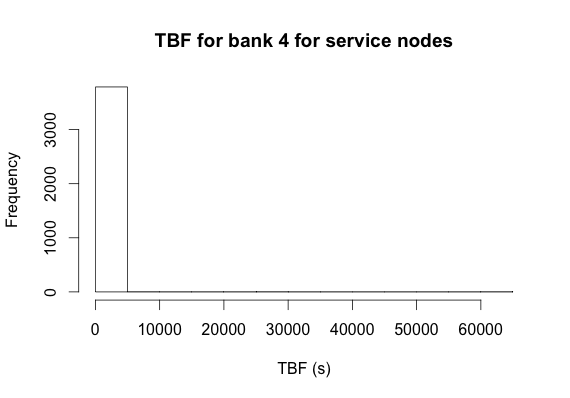
\includegraphics{images/tbf_4_s.png}
\end{figure}

\begin{figure}[h]
\centering
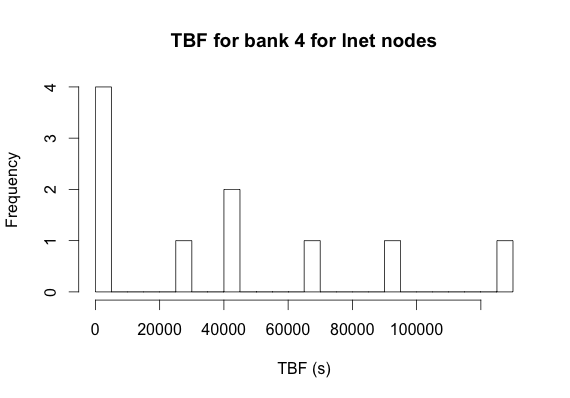
\includegraphics{images/tbf_4_l.png}
\end{figure}

\begin{figure}[h]
\centering
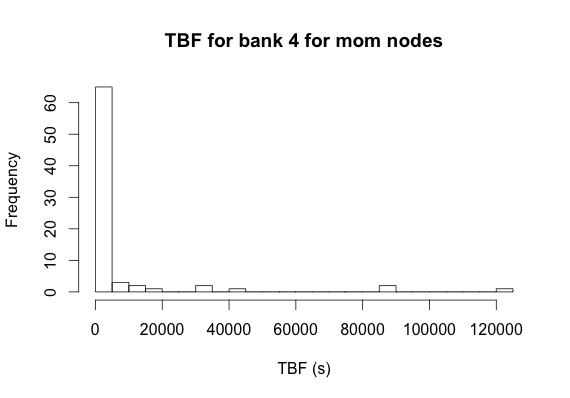
\includegraphics{images/tbf_4_m.png}
\end{figure}

\begin{figure}[h]
\centering
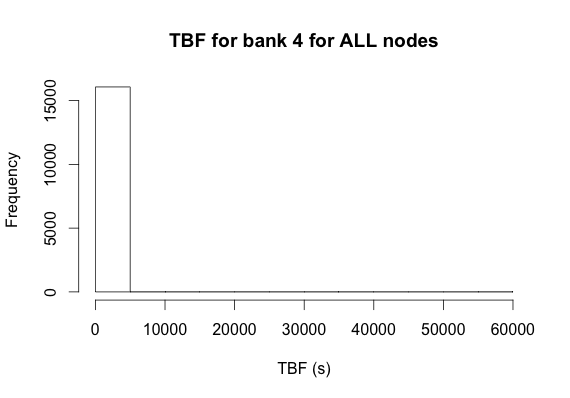
\includegraphics{images/tbf_4_a.png}
\end{figure}

\subsubsection{Plotting the Hazard Rate}

First, note that our hazard rate analysis is necessarily limited by our data set--ideally, we would able to track failures over the entire lifetime of the hardware.  Given these circumstances, we decided to shift our timestamp data to define our origin time as the start of October 6 (12:00 AM CDT) and run \fix{muhaz} on this data.

The hazard rate plots are shown below:

\subsubsection{Analysis}

We derived the following insights based on our results:

\begin{itemize}
\item The MTBF for each day does not appear to be comparable across banks for different days.  We believe that this could be the case because of the relatively small size of our data set; as a result, noise due to other factors (system load, for example) dominated any other trends in the data.  One small trend is that Saturdays (days 0 and 7) appeared to have higher MTBFs than other data throughout the week, but we are not sure if this trend is statistically significant.
\item The time between failures appears to trend significantly towards small numbers.  We believe that one reason that this occurs is because failures may occur more often during heavy use; if a failure happens, the machine is more likely to be under more load, so more failures are likely to follow.  Similarly, permanent hardware failures and cosmic ray strikes are likely to be localized to a small area, and processors tend to access physically-close regions of memory over a short period of time; as a result, when a failure occurs, other failures should be likely to occur in a short time.
\item The hazard rate generally increases as time goes on.  In a general case, this occurs because components are worn out by use and fail naturally over time.  However, as 8 days is an extremely short period of time, we believe that these graphs are more of a consequence of \fix{muhaz}'s graphing methodology than any particular trend. 
\end{itemize}

\section{Task 2}

\subsection{Breakdown of the memory errors \% in Single, dual, triple, quadruple bit errors}

To determine the number of bits in a memory error, we looked up the
corresponding syndrome in the syndrome table.  Once the entry is located, we
check the error bitmask and count the number of `1's in the bitmask.  This
number tells us the number of bits in error when that syndrome was
reported\cite{AMD_BKDG}.  We calculated the number of bits per error for all
memory errors, gathered results and calculated the distribution across machine
type. The results of this study are presented in Table \ref{tab:mem_breakdown}

% latex table generated in R 3.0.2 by xtable 1.7-1 package
% Sun Mar  2 01:04:22 2014
\begin{table}[ht]
\centering
\caption{Memory Error Percentage Breakdown by number of bits and machine type}
\label{tab:mem_breakdown}
\begin{tabular}{rrrrrrr}
  \hline
 & compute & GPU & lnet & service & mom & ALL \\
  \hline
1 & 86.79 & 92.09 & 100.00 & 99.87 & 82.00 & 89.72 \\
  2 & 5.48 & 2.36 & 0.00 & 0.13 & 18.00 & 4.28 \\
  3 & 2.18 & 0.84 & 0.00 & 0.00 & 0.00 & 1.66 \\
  4 & 2.51 & 3.20 & 0.00 & 0.00 & 0.00 & 2.02 \\
  5+ & 3.03 & 1.52 & 0.00 & 0.00 & 0.00 & 2.32 \\
   \hline
\end{tabular}
\end{table}

From table \ref{tab:mem_breakdown}, we can make a few important observations regarding the data:
\subsubsection{Multibit errors are significant:} Roughly 10\% of all memory
errors are multibit errors.  It should also  

\subsubsection{Chipkill is extremely effective:}  There was only one
uncorrectable memory error in our dataset, but there were 11633 corrected
errors.  Again, 10\% of those were multibit and were therefore corrected.  If
the behavior exhibited during these 8 days was representative of a year, we
could expect around 55,000 multibit errors per year. Having that many
uncorrectable errors in a year would be unacceptable in nearly any environment
(except perhaps a stateless web server farm).  Therefore, Chipkill is not only
beneficial for a system like Blue Waters, but necessary.

\subsubsection{Compute nodes exhibit the largest percentage of multibit
errors:} While compute nodes had a lower percentage of multibit errors (on
average) in our dataset, it is difficult to tell if that trend would extend
across the full dataset.  Since GPU and service nodes have half of the DIMMs
present in compute nodes, the number of multibit errors may be undersampled in
our eight day dataset.

\subsection{How frequent (time) are multiple (>1) bit errors?}

Fig. \ref{fig:mem_error_per_hr} plots the number of memory errors per hour for
each machine type.  In this figure, it is easy to see that memory errors in 
compute nodes clearly dominate.  However, this trend could be attributed to the
large number of compute nodes (22640) compared to the fewer GPU (4192) and
service (1936) nodes.  Therefore, this figure was normalized to the number of
node types in Fig. \ref{fig:mem_error_per_hr_normed}.  In this plot, all of the
rates differ by orders of magnitude.  For such a small dataset, it is easy for a
few nodes to dominate.  However, one could still expect different node types to
behave differently as all of these types differ in the way they use memory.

\begin{figure}[h]
  \centering
  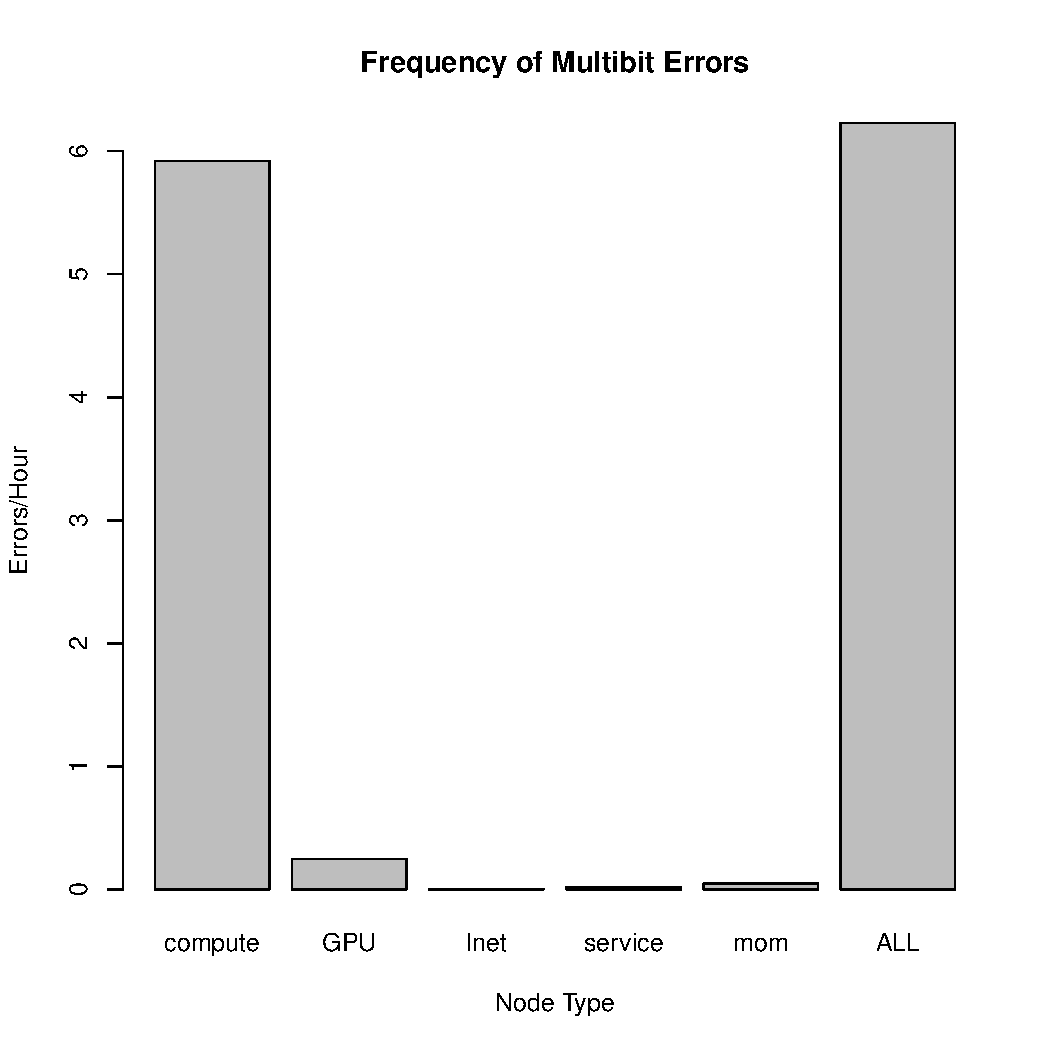
\includegraphics[width=0.45\textwidth]{images/task2_2}
  \caption{Bar graph for the number of Memory errors/hour for each machine
  type.}\label{fig:mem_error_per_hr}
\end{figure}

\begin{figure}[h]
  \centering
  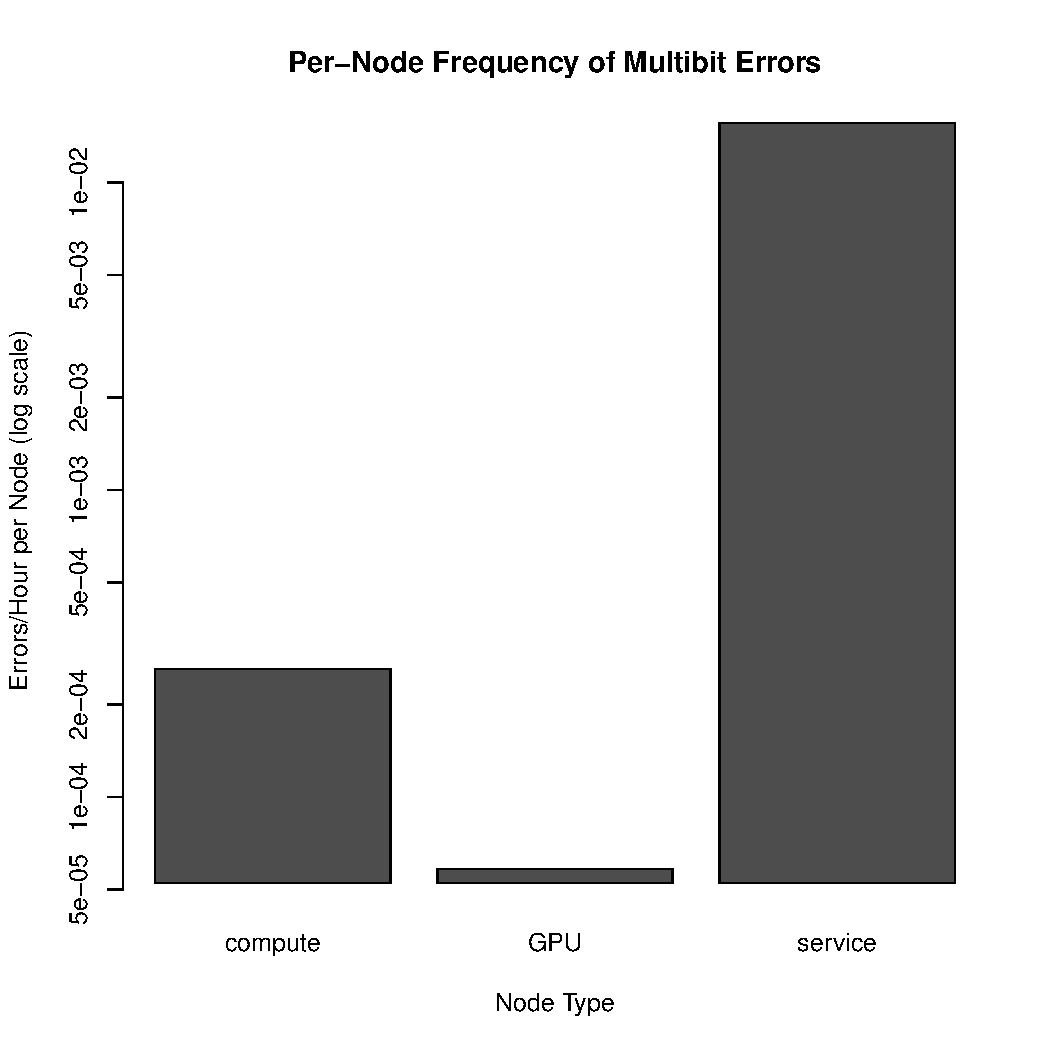
\includegraphics[width=0.45\textwidth]{images/task2_2_normed}
  \caption{Bar graph for the number of Memory errors/hour for each machine
  type, normalized to the number of nodes in each
  type.}\label{fig:mem_error_per_hr_normed}
\end{figure}

\subsection{How many uncorrectable errors would Blue Waters have if using only ECC? How effective is Chipkill wrt ECC?}

If Blue Waters had only ECC, it would not be able to correct any multibit
errors, so errors in more than one bit would become uncorrectable.  There were
1196 errors that would have become uncorrectable without Chipkill.  This makes
Chipkill extremely effective and the data here present a strong case for
Chipkill being mandatory in a system of this size.

A table comparing the same system with and without Chipkill is shown in Table
\ref{tab:mem_fit_mtbf}.
\begin{table}[ht]
\centering
  \begin{tabular}{rrr}
  \hline
  & FIT/Mbit & MTBF \\ 
  \hline
  Chipkill & 0.00039 & 192.00 \\ 
  No Chipkill & 0.47150 & 6.23 \\ 
  \hline
\end{tabular}
\caption{FIT/Mbit and MTBF. One FIT = 1 Failure in $10^9$ hours, MTBF is in
hours.}
\label{tab:mem_fit_mtbf}
\end{table}

In Table \ref{tab:mem_fit_mtbf}, we present the MTBF and FIT/Mbit for Blue
Waters given our dataset.  Again, Chipkill demonstrates its value and is
indispensable for a system of this size.   Here, we present FIT/Mbit so that
we can compare with the study in \cite{schroeder2009dram}.  To calculate
FIT/Mbit, we counted the number of uncorrectable errors (with and without
Chipkill) and used the following formula:
\begin{equation*}
  FIT = \frac{10^9N_{\textrm{failures}}}{(1614080\cdot8\cdot1024)t}
\end{equation*}
, where $N_{\textrm{failures}}$ is the number of failures for that environment,
$t=8\cdot24$ is the timespan of the data set in hours and the system has
1614080GiB of memory and there are $8\dot1024$ GiB to a Mbit. In the
aforementioned study, the authors found an average of 778--25,000 FIT/Mbit for
their systems (ECC only DDR DIMMs).  The values calculated here are
significantly, but the authors of \cite{schroeder2009dram} cite that previous
lab studies showed DRAM to exhibit < 1 FIT/Mbit.  The MTBF without Chipkill
becomes significantly smaller since with Chipkill there was only one
uncorrectable error.

\section{What is the percentage of faulty DRAM?  (i.e., DRAM with permanent
memory faults) }

\subsection{How can you spot them in your dataset?}
We attempt to follow industry standard practices and consider any DIMM that
would warrant an in-the-field replacement as ``faulty.''  The two criteria used
are: (1) if the DIMM has any uncorrectable errors (2) if the number of
correctable errors per unit time exceeds a certain threshold.  For criteria (1),
there was only one machine in the dataset that satisfied the requirement.  To
set an appropriate threshold for (2), we again looked at the study in
\cite{schroeder2009dram}.  The authors found that on average, 3351--4530
correctable errors were experienced per year.  Thus, we determined that memory
exhibiting 5000 or more correctable errors per year (scaled to our dataset) is
faulty with a rather high degree of confidence.

%assumptions, multiple DIMMs, interleaving unsure - assume that two DIMMs don't
%fail on the same system.  since a rare event, Should not skew data and average out.

\section{Task X}
\subsection{What you want to analyze}
We analyzing the rest of the data, we noticed that some machines had multiple
error types.  We estimated that these nodes had a larger problem, such as a
faulty motherboard.

\subsection{Why that is important}
If one is not careful and sees a series of memory errors, it is possible to keep
installing new memory when it is not the culprit.  Also, as motherboard
components tend to handle communication with I/O devices, there could be a
concern about silent data corruption or possible fault propagation. 

\subsection{What are your findings}
Fig. \ref{fig:taskx} contains a histogram that counts the nodes by 
the number of error types they exhibit in the sample dataset.  One can see that
while the number of machines with each error type decays exponentially, there
are still machines with three or more types of errors.  These machines likely
have a CPU/motherboard problem.  In Fig. \ref{fig:taskx_types}, we plot the
number of errors caused by machines against their number of error types.  Here,
it is clear that even though machines with 4 or 5 error types are the minority
in terms of nodes with errors, they represent a little less than half of all
errors generated.
\begin{figure}[h]
  \centering
  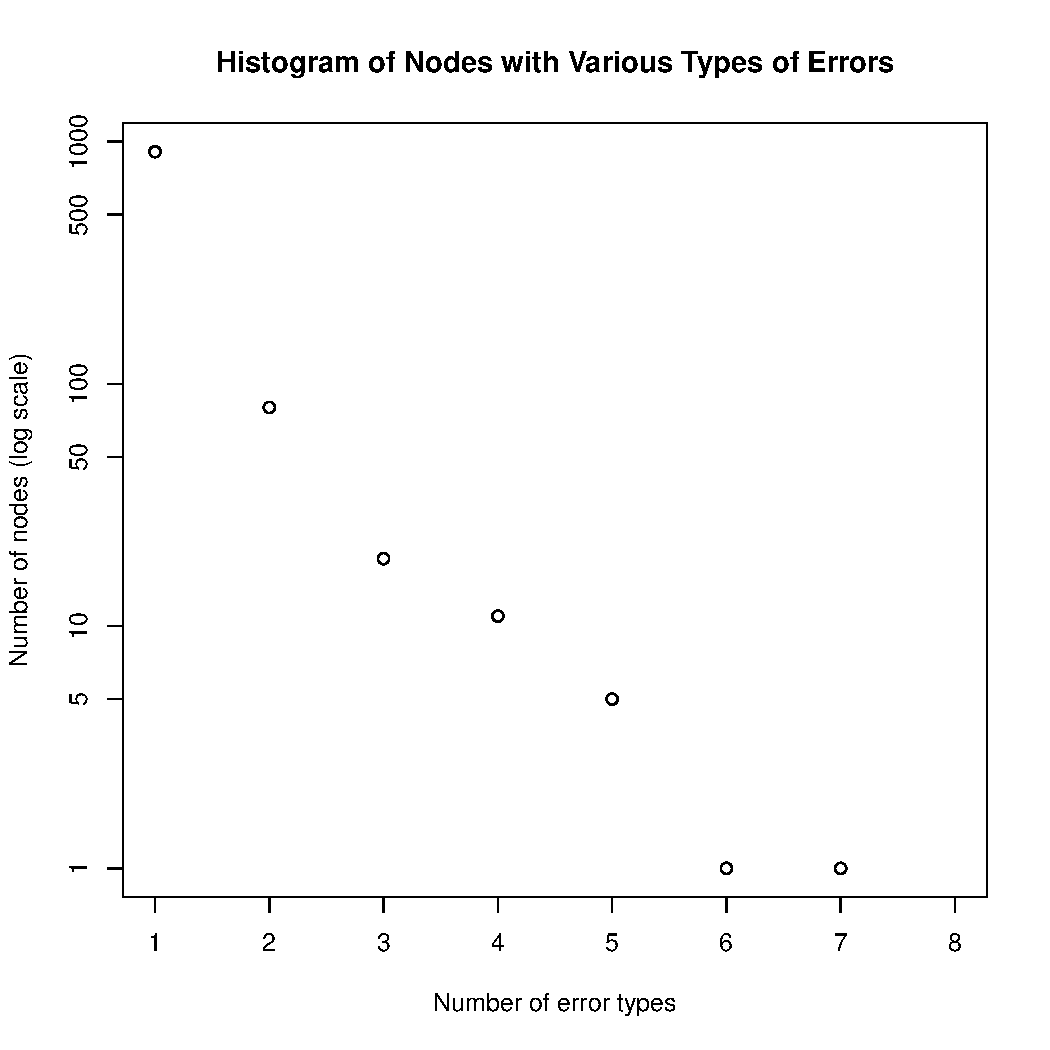
\includegraphics[width=0.45\textwidth]{images/taskx}
  \caption{Histogram of number of error types per nodes. The y axis is a log
  scale}\label{fig:taskx}
\end{figure}
\begin{figure}[h]
  \centering
  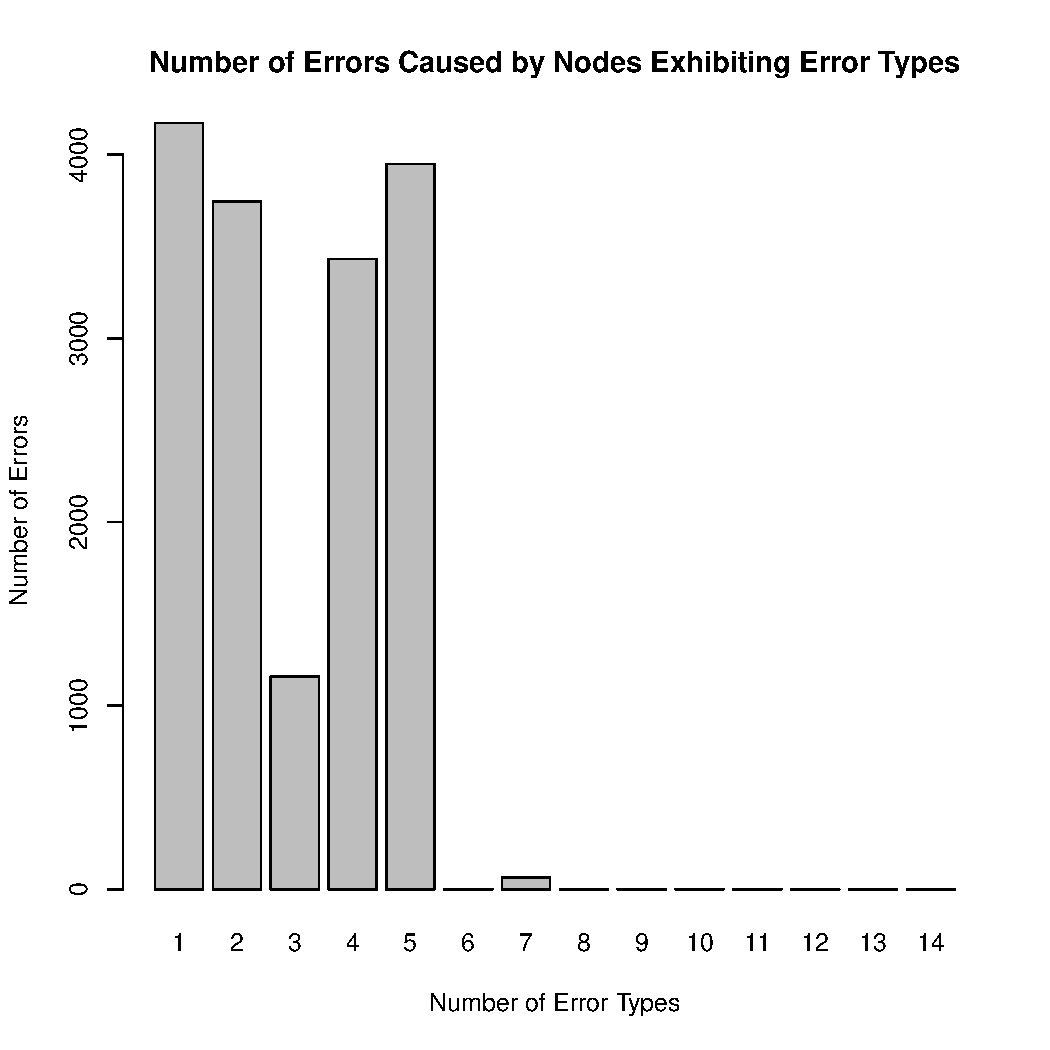
\includegraphics[width=0.45\textwidth]{images/task_x_types}
  \caption{Number of errors caused by nodes experiencing that many error types.
  }\label{fig:taskx_types}
\end{figure}


\section{Final Notes}
\begin{itemize}
  \item The code is included in this zip file with names like ``task1.R'' for
  tasks and general function names for more library-like files
  \item Since all plots involved at most one line at a time, legends were
  omitted for legibility.
\end{itemize}

%\section*{acknowledgments}

\bibliographystyle{IEEEtran}
\bibliography{ece542_group8}

%\clearpage
%\onecolumn
%\section{Code}
%\lstset{
%  language=Python,
%  showstringspaces=false,
%  formfeed=\newpage,
%  tabsize=2,
%  commentstyle=\itshape,
%  basicstyle=\ttfamily,
%  morekeywords={models, lambda, forms},
%  %basicstyle=\ttm,
%  %keywordstyle=\ttb\color{deepblue},
%  %otherkeywords={self},             % Add keywords here
%  %emph={Event,__init__},          % Custom highlighting
%  %emphstyle=\ttb\color{deepred},    % Custom highlighting style
%  %stringstyle=\color{deepgreen},
%}
\end{document}
